\documentclass[11pt,a4paper]{article}
\usepackage[a4paper,margin=0.83in,headheight=22pt,footskip=24pt]{geometry}
\usepackage[T1]{fontenc}
\usepackage{lmodern}
\usepackage{microtype}
\usepackage{amsmath,amssymb,mathtools,bm}
\usepackage{graphicx}
\usepackage{booktabs,tabularx,array,longtable,multirow}
\usepackage[table]{xcolor}
\usepackage{enumitem}
\usepackage{float}
\usepackage{caption}
\usepackage{subcaption}
\usepackage{fancyhdr}
\usepackage[backend=biber,style=numeric-comp,sorting=none,natbib=true]{biblatex}
\renewcommand*{\bibfont}{\small}\setlength{\bibitemsep}{2pt}\setlength{\bibparsep}{0pt}
\addbibresource{paper.bib}
\usepackage{hyperref}
\usepackage[nameinlink,noabbrev]{cleveref}
\hypersetup{colorlinks=true,linkcolor=teal!55!black,citecolor=teal!55!black,urlcolor=teal!65!black,pdftitle={Silica Light Meters: Physics-Constrained Inverse Learning of Past Underwater Light Regimes from Diatom Frustule Photonic Crystals},pdfauthor={Devanik Debnath}}
\definecolor{ink}{HTML}{19324A}
\definecolor{teal}{HTML}{197C83}
\definecolor{slate}{HTML}{64748B}
\definecolor{mist}{HTML}{EEF4F5}
\definecolor{gold}{HTML}{C08A38}
\captionsetup{font=small,labelfont={bf,color=ink},skip=6pt}
\setlength{\parskip}{4.1pt}
\setlength{\parindent}{0pt}
\setlist[itemize]{leftmargin=1.35em,itemsep=2pt,topsep=3pt}
\setlist[enumerate]{leftmargin=1.55em,itemsep=2pt,topsep=3pt}
\pagestyle{fancy}
\fancyhf{}
\fancyhead[L]{\small\color{slate}SILICA LIGHT METERS}
\fancyhead[R]{\small\color{slate}Research preprint \textbar\ 18 October 2026}
\fancyfoot[C]{\small\thepage}
\renewcommand{\headrulewidth}{0.4pt}
\renewcommand{\headrule}{\hbox to\headwidth{\color{teal}\leaders\hrule height \headrulewidth\hfill}}
\newcommand{\E}{\mathcal{E}}
\newcommand{\Tfr}{\mathcal{T}}
\newcommand{\Kphy}{\mathbf{K}_{\!\mathrm{phy}}}
\newcommand{\Rtwo}{R^2}
\newcommand{\dd}{\,\mathrm{d}}
\title{\vspace{-1.1cm}\begin{flushleft}\large\color{teal}\textsc{Theoretical and Computational Research}\end{flushleft}\vspace{0.35em}{\LARGE\bfseries\color{ink} Silica Light Meters:\\[0.2em] Physics-Constrained Inverse Learning of Past Underwater Light Regimes from Diatom Frustule Photonic Crystals}}
\author{\textbf{Devanik Debnath}\\[-0.1em]\small Department of Electronics and Communication Engineering\\\small National Institute of Technology Agartala, India\\[0.2em]\small Research-process coordination: Xylia}
\date{\small Research preprint and synthetic methods demonstration \textbar\ 18 October 2026}
\begin{document}
\maketitle
\vspace{-0.4em}
\begin{center}\color{teal}\rule{0.92\linewidth}{1.0pt}\end{center}
\begin{abstract}
Diatom frustules are hierarchically porous silica structures with species-dependent diffraction and light-trapping properties. Those optical phenomena are established; using them to infer past underwater irradiance is not. A direct inversion from fossil pore geometry to historical light is vulnerable to several non-identifiabilities: the same geometry can occur under different ecological conditions, evolutionary history induces trait covariance, and water-column attenuation depends on depth, suspended particles, dissolved matter, mixing and ice cover. We formulate a falsifiable programme that couples (i) electromagnetic forward calculations of measured frustule geometry, (ii) hierarchical phylogenetic models of species-level morphology and measured light preference, (iii) wavelength-dependent water-column radiative transfer, and (iv) an uncertainty-aware inverse model for sediment-core reconstruction. The primary first test is deliberately narrow: does a physics-derived spectral-response descriptor predict independently measured species light preference better than raw pore size after coarse phylogenetic and habitat controls, under held-out-taxon evaluation? A synthetic pipeline is implemented to stress-test feature generation, confounding, validation logic and inverse non-uniqueness. It does not solve Maxwell's equations, use an empirical species dataset, fit a real phylogeny, or reconstruct a real lake. Its numerical results are therefore software and identifiability demonstrations only, not evidence that frustules preserve a recoverable pale-light signal. We specify controls, baselines, uncertainty tests, independent core validation, and outcomes that would falsify the central proposal. The defensible contribution is a physics-informed validation architecture and an explicit go/no-go test, not a demonstrated paleoclimate proxy.
\end{abstract}
\vspace{-0.3em}
\textbf{Keywords:} diatoms; biosilica; frustule; photonic structures; inverse problems; phylogenetic comparative methods; paleolimnology; physics-informed machine learning; uncertainty calibration

\section{Research question and contribution}
A robust paleoproxy must encode a past environmental process, be measured reproducibly, remain interpretable under the archive's preservation process, and predict an independent target better than simpler alternatives. The proposed ``Silica Light Meters'' programme asks whether optical computations on diatom frustule geometry can add predictive information about historical underwater light regimes beyond raw pore measurements and established assemblage-based indicators.

The gap is not that diatom silica interacts with light. Experiments and numerical models have demonstrated diffraction, wavelength-dependent concentration and light trapping in frustules, including calculations using rigorous coupled-wave analysis (RCWA) and finite-difference time-domain (FDTD) methods \citep{ferrara2014,chen2015,romann2015}. Nor is it new to infer environmental conditions from diatom morphology: Welchans examined pore size in \textit{Aulacoseira crenulata} in one Amazon lake and reported an indirect relationship with light availability, and work on \textit{Fragilariopsis kerguelensis} related morphotype abundance and valve shape to reconstructed and modern sea-surface temperatures \citep{welchans2020,kloster2018,glemser2019}. The proposed contribution is narrower: connect a measured geometry to a physically computed spectral response, place that response inside a phylogenetically controlled ecological model, and test incremental out-of-sample skill under explicit nuisance variation before treating it as a paleo-light proxy.

\textbf{Primary question.} With taxonomy/phylogeny fixed before analysis, does a morphology-derived optical-response feature improve prediction of measured species light preference over raw pore size and conventional covariates in held-out-taxon validation?

\textbf{Secondary question.} If the first test succeeds, can an uncertainty-calibrated hierarchical inverse model recover a historical light-regime index from core morphometrics while accounting for water-column attenuation, habitat, preservation, chronological uncertainty and phylogenetic dependence?

\textbf{Scope.} This manuscript is a theoretical methods proposal with a synthetic pipeline exercise. There are no new microscopy measurements, growth experiments, taxon-level optical measurements, sediment-core analyses, or paleoclimate reconstructions here. No field data or biological outcomes are reported.

\begin{table}[H]
\caption{Claim boundary and epistemic status. This table is a release safeguard, not a novelty score.}
\label{tab:claims}
\small\begin{tabularx}{\linewidth}{@{}p{0.24\linewidth}p{0.27\linewidth}X@{}}
\toprule
Claim & Status & What would be needed to upgrade it \\
\midrule
Frustules can shape/diffract light in wavelength-dependent ways & Established in selected taxa and configurations & Replication across relevant species, geometries and intact/fossil conditions \\
Morphology can covary with environment & Established in selected taxa; not universal & Independent calibration across species, habitats and environmental gradients \\
A computed spectral descriptor beats pore size after phylogenetic control & Untested hypothesis & Measured geometry and light-preference data; held-out-taxon improvement \\
A core-based posterior can recover past light & Proposed inference programme & Independent core target, nuisance controls, chronology and calibrated uncertainty \\
A deep-time frustule functions as a literal light meter & Not established; avoid as a factual description & Mechanistic evidence that the proxy pathway persists through evolution, burial and preservation \\
\bottomrule
\end{tabularx}
\end{table}

\section{What is established, and what remains open}
\subsection{Optics of a frustule}
A frustule is a hydrated silica shell whose hierarchical pores, slits and layers can modify transmission and near-field intensity. Ferrara \textit{et al.} measured optical features of \textit{Arachnoidiscus} valves and reported spatially separated intensity patterns; Chen \textit{et al.} used RCWA and FDTD and compared simulated light-trapping behaviour with optical measurements; a further study reported wavelength- and orientation-dependent capture in \textit{Coscinodiscus centralis} \citep{ferrara2014,chen2015,romann2015}. These findings justify computing a spectral response from measured geometry. They do not imply that one scalar pore dimension maps uniquely to the light conditions in which the organism grew.

\subsection{Morphology as an ecological and paleoenvironmental signal}
The closest direct precedent is Welchans' undergraduate thesis on \textit{A. crenulata} at Lake Garzacocha, Amazonia. It reports an indirect relationship between pore size and light availability and explicitly recommends testing additional communities and locations \citep{welchans2020}. Separately, Kloster \textit{et al.} identified two \textit{F. kerguelensis} morphotypes in sediment by valve rectangularity and reported morphotype-abundance relationships with reconstructed sea-surface temperature; Glemser \textit{et al.} investigated those morphotypes in recent assemblages and found a geographic/environmental cline, while noting the need for broader sampling \citep{kloster2018,glemser2019}. Thus morphology-based environmental inference is established as a research strategy. The open question here is whether optical simulation adds a transferable, mechanistically interpretable descriptor rather than repackaging existing morphometrics.

\subsection{The ecological channel is not the optical channel}
Optical response describes how a structure interacts with incident illumination. Ecological selection describes how traits or taxa become more or less prevalent under environmental conditions over development and generations. These are separate mappings. A forward electromagnetic calculation cannot by itself infer the environment that selected the geometry. The proposed model must estimate both mappings and account for plausible alternatives such as nutrient supply, temperature, salinity, growth phase, silicification, turbulence and substrate.

\begin{figure}[H]
\centering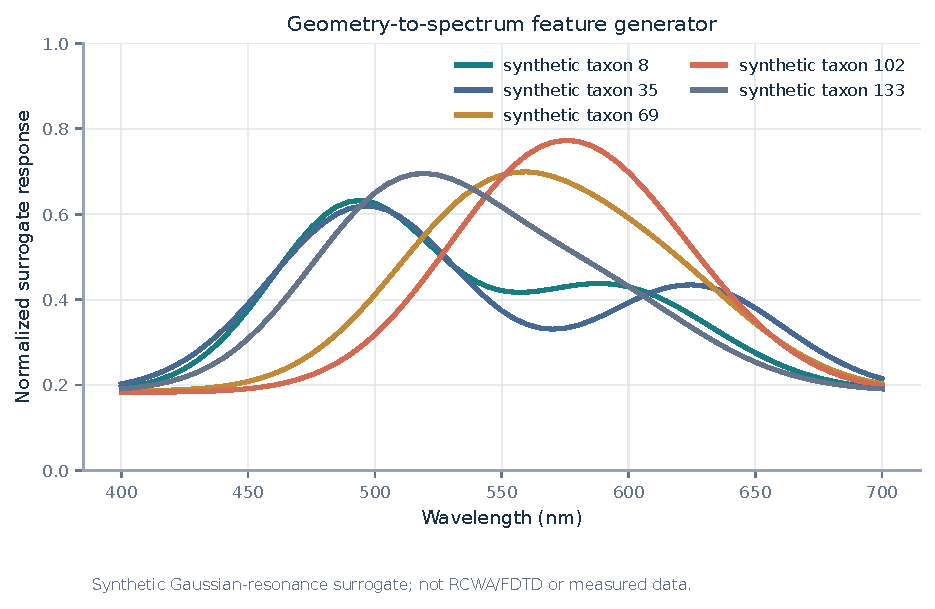
\includegraphics[width=0.96\linewidth]{figures/fig01_surrogate_spectra.pdf}
\caption{Illustrative surrogate spectral responses for hypothetical geometries. These curves are generated by a simple Gaussian-resonance function for software and feature-pipeline tests; they are not RCWA/FDTD outputs or measured frustule spectra.}
\label{fig:spectra}
\end{figure}

\section{Forward model: from geometry to aquatic light exposure}
\subsection{Frustule optical response}
Let $g_s$ denote a vector of geometry measurements for species $s$ (pore pitch, pore diameter, porosity, layer thickness, symmetry and surface orientation), $n(\lambda)$ the wavelength-dependent complex refractive index, and $\theta$ incident orientation/polarization. The desired forward solver returns a transmittance or absorptance response
\begin{equation}
\Tfr_s(\lambda,\theta)=\mathcal{M}\!\left(g_s,n(\lambda),\theta;\lambda\right),
\label{eq:forward}
\end{equation}
where $\mathcal{M}$ is a validated Maxwell-equation solver such as RCWA for an approximately periodic unit cell, with FDTD or another method used for finite, disordered or strongly three-dimensional structures. The optical model must be checked against measured spectra for representative taxa; periodic-cell assumptions should not be silently imposed on irregular structures.

The descriptor should retain the full spectral response where feasible rather than collapsing it immediately into a pore-size surrogate. Candidate summaries include a vector of band-integrated responses, spectral centroid, peak locations, polarization/orientation sensitivity, and an overlap between the frustule response and a specified action spectrum. These summaries are features, not direct measurements of historical irradiance.

\subsection{Underwater radiative transfer}
For downwelling spectral irradiance $\E_0(\lambda,t)$ just below the surface, a first-order attenuation model is
\begin{equation}
\E(\lambda,z,t)=\E_0(\lambda,t)\exp\!\left[-K_d(\lambda,t)z\right],
\label{eq:beer}
\end{equation}
where $z$ is depth and $K_d$ is the wavelength-dependent diffuse attenuation coefficient. Equation~\eqref{eq:beer} is a useful reduced model, not a universal description of radiative transfer; scattering geometry and the distinction between direct and diffuse irradiance may require a fuller model. Measurements in shallow turbid lakes have shown that the Beer--Lambert approximation can be adequate while its residuals still depend on wavelength-specific conditions and water-quality constituents \citep{weiskerger2018}. The model should include suspended mineral and organic particles, colored dissolved organic matter, chlorophyll, mixing and under-ice boundary conditions where relevant.

A frustule-level optical exposure index can be defined as
\begin{equation}
Q_s(t,z)=\int_{\lambda_{\min}}^{\lambda_{\max}}\E(\lambda,z,t)\,\Tfr_s(\lambda,\theta)\,A_s(\lambda)\dd\lambda,
\label{eq:exposure}
\end{equation}
where $A_s(\lambda)$ is an empirically motivated biological action weighting or a clearly identified neutral weighting. The integral is only a candidate bridge between optics and physiology. In an experiment, it must be compared with growth, photosynthetic yield or another pre-specified preference outcome; it cannot be interpreted as fitness without that link.

\begin{figure}[H]
\centering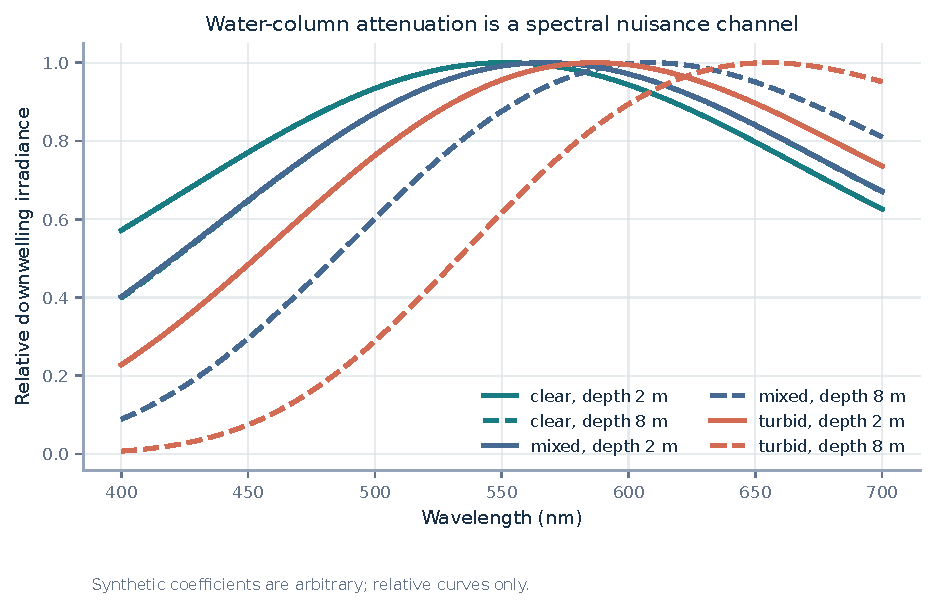
\includegraphics[width=0.96\linewidth]{figures/fig02_attenuation.pdf}
\caption{Wavelength-dependent synthetic attenuation at two depths under three illustrative water types. Curves demonstrate a nuisance mechanism only; coefficients are arbitrary and are not environmental estimates.}
\label{fig:attenuation}
\end{figure}

\begin{table}[H]
\caption{Core variables and the measurement or assumption required for each.}
\label{tab:variables}
\small\begin{tabularx}{\linewidth}{@{}p{0.17\linewidth}p{0.28\linewidth}X@{}}
\toprule
Symbol & Meaning & Status / acquisition path \\
\midrule
$g_s$ & Frustule geometry & SEM/TEM or calibrated 3-D microscopy; segmentation uncertainty must be propagated \\
$\Tfr_s(\lambda,\theta)$ & Spectral optical response & RCWA/FDTD calibrated to measured spectra; no empirical values in this paper \\
$\E_0(\lambda,t)$ & Surface spectral irradiance & In situ spectral sensors or instrumented analogue sites \\
$K_d(\lambda,t)$ & Water attenuation & Measured profiles plus optical/water-quality model \\
$Y_s$ & Species light preference / performance & Controlled light-gradient experiment with independent biological readout \\
$u_s$ & Phylogenetic random effect & Fixed, versioned tree with taxonomy uncertainty documented \\
$h_s$ & Habitat / ecology covariates & Temperature, nutrients, salinity, mixing, substrate, depth and growth state \\
$m_{s,t}$ & Preservation/measurement channel & Dissolution, breakage, diagenesis, reworking and sediment mixing estimates \\
$L_t$ & Latent historical light-regime state & Target posterior; identifiable only relative to calibrated response and nuisance model \\
\bottomrule\end{tabularx}
\end{table}

\section{Inverse problem with ecological and phylogenetic structure}
\subsection{Species-level calibration}
Let $Y_{is}$ denote replicate light-preference outcome $i$ for taxon $s$, measured along a controlled irradiance gradient. A hierarchical model can be written as
\begin{equation}
Y_{is}=\alpha+\bm{\beta}^{\top}\bm{\psi}(g_s)+\bm{\gamma}^{\top}h_{is}+u_s+b_{\mathrm{site}(i)}+\epsilon_{is},
\label{eq:hier}
\end{equation}
where $\bm{\psi}(g_s)$ contains a pre-specified set of optical-response features and conventional morphometrics, $h_{is}$ are environmental covariates, $u=(u_1,\ldots,u_S)^\top$ captures phylogenetic dependence, and $b_{\mathrm{site}}$ is a site/batch effect. A standard comparative structure is
\begin{equation}
u\sim\mathcal{N}(0,\sigma^2_{\mathrm{phy}}\Kphy),\qquad\epsilon_{is}\sim\mathcal{N}(0,\sigma^2),
\label{eq:phylo}
\end{equation}
where the covariance $\Kphy$ derives from a documented tree and evolutionary covariance assumption. This covariance is an assumption to assess, not a magical correction for ancestry. For categorical preferences or nonlinear dose-response, the likelihood and link function must match the measured endpoint.

The main confirmatory comparison is deliberately nested: (M0) ecological covariates plus phylogeny; (M1) M0 plus raw pore diameter/porosity; (M2) M0 plus pre-registered optical spectral features. An expanded model (M3) may combine morphology and optical features, but M3 is secondary until multiplicity and model selection are controlled. All transformations and features are frozen before outer test data are examined.

\subsection{Posterior reconstruction in a sediment core}
For core interval $t$, let $\bm{x}_t$ summarize the target light regime (e.g., a spectral centroid and a log-intensity index), $\bm{c}_t$ summarize nuisance environmental states, and $\bm{r}_t$ summarize observed taxon/morphology composition. One proposed observation model is
\begin{equation}
p(\bm{r}_t\mid\bm{x}_t,\bm{c}_t,\mathcal{T},m_t)=\mathrm{Multinomial}\!\left(N_t,\bm{\pi}_t\right),
\label{eq:core}
\end{equation}
with
\begin{align}
\mathrm{logit}(\pi_{st})={}&\alpha_s+f_s(\bm{x}_t;\Tfr_s)+\bm{\gamma}_s^\top\bm{c}_t+u_s+m_{st}.
\label{eq:composition}
\end{align}
Here $f_s$ must be trained against measured ecological outcomes; one must not set it equal to $Q_s$ without validation. A state-space prior can describe temporal smoothness in $\bm{x}_t$ and $\bm{c}_t$, but posterior smoothness is regularization, not independent evidence. When nuisance states are weakly observed, return a broad or multimodal posterior and a non-identifiability warning rather than a precise-looking point estimate.

\subsection{An identifiability condition}
A local linearization of expected observations around candidate state $(\bm{x},\bm{c})$ gives
\begin{equation}
\Delta\bm{\mu}\approx J_x\Delta\bm{x}+J_c\Delta\bm{c},
\label{eq:jac}
\end{equation}
where $J_x$ and $J_c$ are Jacobians for target and nuisance variables. If columns of $J_x$ lie in or near the column space of $J_c$, then changes in target light can be mimicked by changes in nuisance state. For the whitened observation model, the relevant target information after linearly projected nuisance effects can be summarized by
\begin{equation}
\mathcal{I}_{x\mid c}=J_x^\top W^{1/2}(I-P_{W^{1/2}J_c})W^{1/2}J_x,
\label{eq:info}
\end{equation}
where $W$ is an observation-precision matrix and $P_A$ is the orthogonal projector onto the columns of $A$. A nearly singular $\mathcal{I}_{x\mid c}$ indicates that at least one target direction is poorly identified. This is a local diagnostic, not a complete proof of global identifiability. Synthetic examples in this paper use this idea to show why a one-number ``pore-size thermometer'' should not be trusted.

\begin{figure}[H]
\centering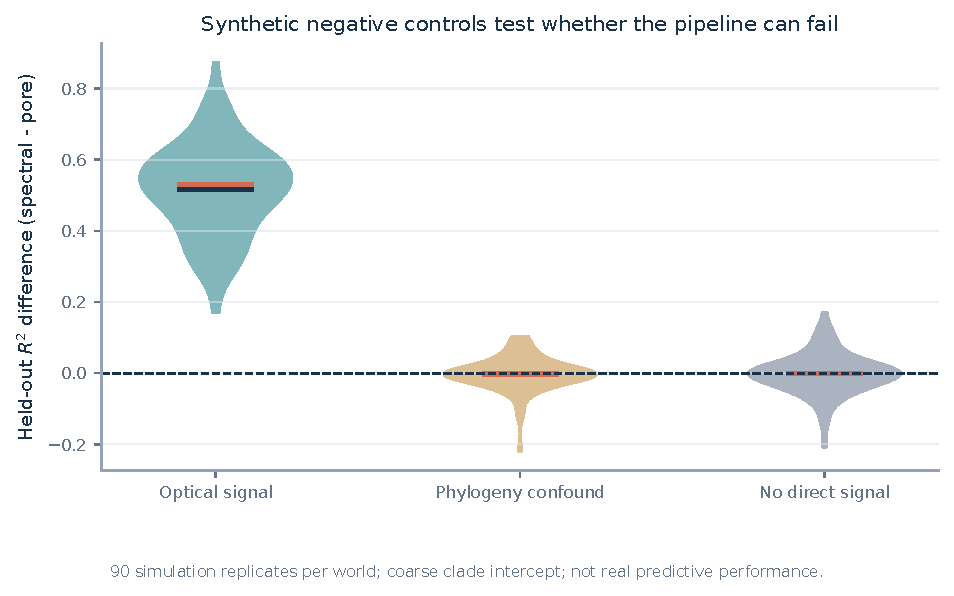
\includegraphics[width=0.95\linewidth]{figures/fig03_incremental_prediction.pdf}
\caption{Synthetic diagnostic of incremental predictive value after a coarse clade intercept. For each simulated world, the plot compares held-out-taxon $R^2$ for a spectral surrogate feature and raw pore diameter. Replicates are generated from explicitly defined toy mechanisms; distributions are not empirical performance estimates.}
\label{fig:benchmark}
\end{figure}

\begin{figure}[H]
\centering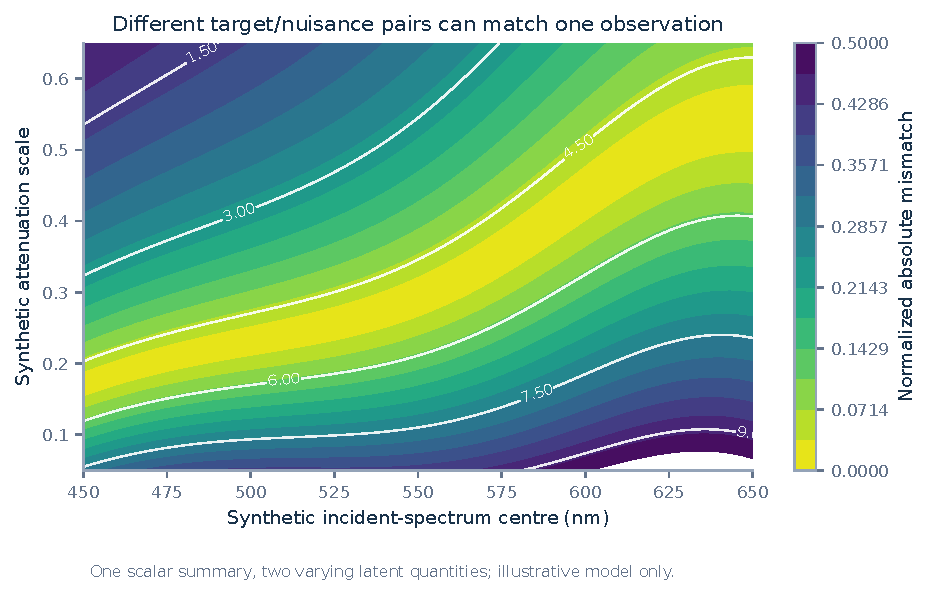
\includegraphics[width=0.92\linewidth]{figures/fig04_inverse_nonidentifiability.pdf}
\caption{Synthetic inverse ambiguity: combinations of spectral-light centre and attenuation strength can yield similar scalar observations. A precise posterior cannot be justified when multiple nuisance/target combinations produce effectively the same measurement.}
\label{fig:inverse}
\end{figure}

\section{Phylogenetic and ecological controls}
Diatom taxonomy has historically relied heavily on valve morphology; molecular phylogenies have repeatedly revised how morphological groups map to evolutionary history. A 2026 phylogenetic classification paper emphasizes that traditional groupings do not always represent monophyletic evolutionary units \citep{kociolek2026}. Therefore the analysis must not treat taxonomic labels as error-free independent samples or use the same morphology traits both to build a tree proxy and to claim an independent adaptation signal.

The pre-analysis protocol should: (1) choose a versioned phylogeny using molecular data where available; (2) include uncertainty in tree placement for poorly sampled taxa; (3) include clade random effects and, as a sensitivity analysis, a Brownian/covariance-based comparative model; (4) control the major measured habitat covariates; (5) hold out taxa, and separately hold out sites or regions, before any feature selection; (6) compare posterior predictive distributions, not only in-sample fit; and (7) test whether the spectral feature adds information beyond pore diameter, porosity, valve dimensions and established assemblage metrics.

\begin{table}[H]
\caption{Closest prior work and what this proposal does not claim as new.}
\label{tab:prior}
\small\begin{tabularx}{\linewidth}{@{}p{0.25\linewidth}p{0.37\linewidth}X@{}}
\toprule
Prior strand & Established contribution & Residual question for this project \\
\midrule
Diatom optics \citep{ferrara2014,chen2015,romann2015} & Measured and modelled wavelength-dependent optical effects, light focusing/trapping & Does a calibrated spectral descriptor add ecological predictive skill across taxa? \\
Single-lake morphology/light thesis \citep{welchans2020} & Pore-size/light relationship explored for one taxon and lake & Does the result generalize under phylogeny, habitat covariates and out-of-site testing? \\
Morphometric paleo-proxies \citep{kloster2018,glemser2019} & Valve morphotypes and environmental gradients linked in a selected species & Is the optical mechanism independently predictive, not just a correlated geometry summary? \\
Diatom paleolimnology \citep{hofmann2020} & Assemblages, depth, substrate and transparency contribute to core interpretations & Can optical features add skill against assemblage baselines and an independent light history? \\
Aquatic light attenuation \citep{weiskerger2018,gordon1989} & Wavelength- and water-quality-dependent attenuation models & Can nuisance uncertainty be separated from the target pale-light trajectory? \\
\bottomrule\end{tabularx}
\end{table}

\begin{figure}[H]
\centering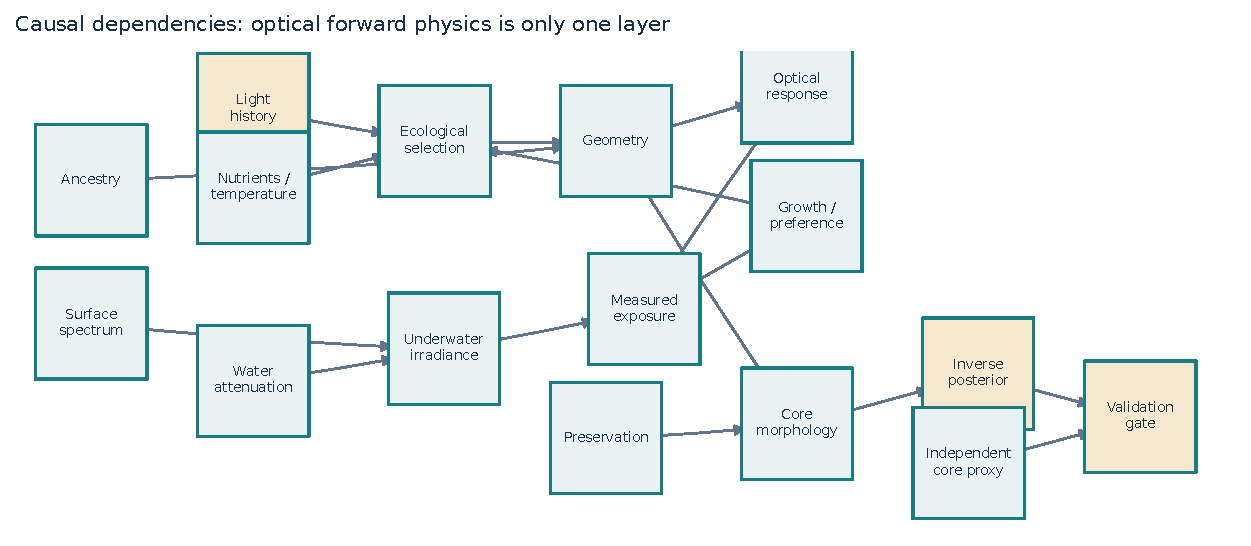
\includegraphics[width=0.91\linewidth]{figures/fig05_causal_graph.pdf}
\caption{Causal dependency graph. The measured optical response is downstream of geometry; ecological morphology also depends on ancestry and non-light habitat factors. The target cannot be inferred from a spectral computation alone.}
\label{fig:causal}
\end{figure}

\begin{figure}[H]
\centering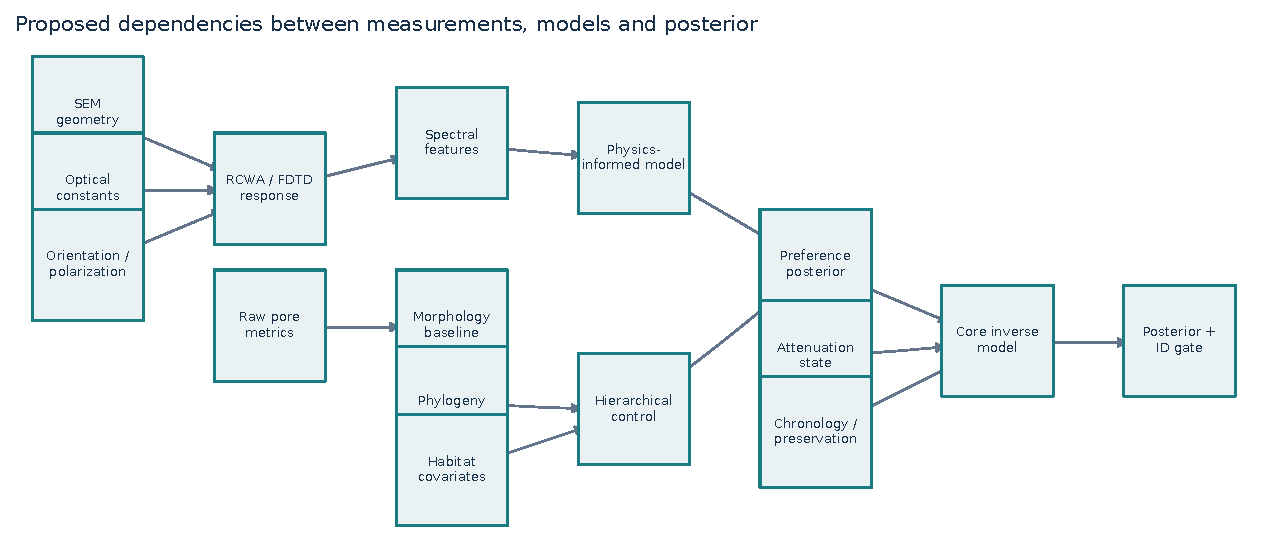
\includegraphics[width=0.90\linewidth]{figures/fig06_feature_graph.pdf}
\caption{Feature-dependency graph separating directly measured geometry, derived optical features, environmental observations and the inferred light regime. Edges represent proposed data and modelling dependencies, not confirmed causal effects.}
\label{fig:features}
\end{figure}

\section{Physics-constrained learning and posterior uncertainty}
The learning component should be modest and testable. Rather than allow a flexible neural model to invent arbitrary geometry-to-light mappings, the forward optical solver defines admissible spectral features and the ecological calibration data define their relation to outcomes. A probabilistic inverse model (or a neural posterior estimator used only after calibration) maps measured morphology and core context to a posterior over light and nuisance regimes. The model should be regularized against contradictions of the forward solver and evaluated against strong non-neural baselines.

Let $q_\phi(\bm{x},\bm{c}\mid\bm{r},\mathcal{G})$ be an approximate posterior conditioned on morphology data $\bm{r}$ and measured geometric inputs $\mathcal{G}$. A suitable objective is a simulation-based calibration objective or a proper scoring rule with an explicit forward consistency penalty:
\begin{equation}
\mathcal{L}(\phi)=\mathcal{L}_{\mathrm{proper}}+\lambda_{\mathrm{fwd}}\mathcal{L}_{\mathrm{forward}}+\lambda_{\mathrm{cal}}\mathcal{L}_{\mathrm{calibration}}.
\label{eq:loss}
\end{equation}
The first term scores predictive distributions on held-out calibrated data; the second penalizes predictions that fail the frozen forward model within its uncertainty; the third targets interval coverage/calibration. The weights are hyperparameters chosen within training folds only. A penalty is not a substitute for a correct likelihood: if the physical model is misspecified, a hard constraint can force a confident error. A sensible implementation therefore propagates optical-constant and segmentation uncertainty and runs sensitivity analyses over model discrepancy.

\begin{table}[H]
\caption{Pre-registered comparison ladder for the first species-level test. The primary contrast is M2 versus M1.}
\label{tab:models}
\small\begin{tabularx}{\linewidth}{@{}p{0.08\linewidth}p{0.28\linewidth}p{0.28\linewidth}X@{}}
\toprule
Model & Predictors & Purpose & Main risk \\
\midrule
M0 & Habitat covariates + phylogenetic effect & Establish ecological baseline & Omitted environment may mimic traits \\
M1 & M0 + pore diameter, porosity, valve dimensions & Strong raw-morphology baseline & Measurement error and collinearity \\
M2 & M0 + frozen optical-response features & Primary candidate model & Forward-model mismatch or spectral overfit \\
M3 & M0 + raw and optical features & Secondary combined model & Extra flexibility; incremental contribution hard to isolate \\
M4 & Assemblage composition / conventional transfer function & Paleo-core benchmark & Depends on modern calibration-set coverage \\
M5 & Permuted response and clade-preserving null models & Negative controls & Null must preserve sampling and dependence structure \\
\bottomrule\end{tabularx}
\end{table}

\section{Synthetic pipeline demonstration}
\subsection{Purpose and assumptions}
The included script \texttt{verify\_model.py} exercises a minimal version of the proposed feature-to-inference workflow. It creates hypothetical taxa across eight clades; samples normalized pore pitch, pore diameter, porosity and layer depth; generates a Gaussian-resonance optical surrogate; and simulates three regimes: an optical-signal world, a phylogenetic-confounding world and a no-direct-signal world. It then compares held-out-taxon prediction using a clade intercept plus a raw pore-size feature against the same clade intercept plus a scalar optical surrogate. The independent splitting procedure is repeated using a fixed master seed.

The toy spectra in \cref{fig:spectra} are not RCWA. The clade intercept is a deliberately coarse control, not a reconstructed diatom phylogeny. The synthetic response is not a measured preference outcome. The numerical experiment demonstrates that the software pipeline can generate feature tables and compare models under a positive-signal scenario and against negative-control scenarios. It cannot demonstrate real predictive skill, phylogenetic robustness, evolutionary adaptation or a historical reconstruction.

\begin{table}[H]
\caption{Observed diagnostic outputs from the fixed-seed synthetic experiment. Values summarize 90 simulated replicates per world; the intervals are the 2.5th and 97.5th replicate quantiles, not empirical confidence intervals.}
\label{tab:synthetic-results}
\small\begin{tabularx}{\linewidth}{@{}p{0.30\linewidth}r r X@{}}
\toprule
Synthetic world & Mean $\Delta R^2$ & Replicate quantiles & Interpretation \\
\midrule
Optical signal & $+0.517$ & $[+0.281,+0.751]$ & The designed optical feature carries signal in this world. \\
Phylogeny-confounded & $-0.001$ & $[-0.105,+0.094]$ & No meaningful incremental signal remains after the coarse clade control. \\
No direct signal & $-0.002$ & $[-0.124,+0.122]$ & The comparison is centred near zero under the negative control. \\
\bottomrule\end{tabularx}
\end{table}

Here $\Delta R^2$ is held-out synthetic prediction $R^2$ for the spectral surrogate minus the raw-pore baseline, both with the same clade-intercept control. The positive-control result is constructed by the data-generating assumptions and should be read as a pipeline sanity check, not a prediction about real species. The two negative controls are equally important: they show that a claimed gain should disappear when the simulator removes the direct effect or makes the association ancestry-confounded.

\subsection{What the synthetic exercise can tell us}
A valid code run must confirm that: transmission surrogates remain in the declared range; depth attenuation is monotone for nonnegative coefficients; the inverse grid is generated from the stated formula; held-out predictions exclude the target taxon's response from fit; and the reported comparisons include all simulated worlds. The key output is not a winning score. It is an audit trail that keeps simulation assumptions visible and makes negative-control scenarios part of the same pipeline.

\begin{table}[H]
\caption{Proposed empirical decision rules. These are preregistration candidates, not results from the synthetic run. Final margins should be justified with pilot precision and frozen before the confirmatory test.}
\label{tab:decisions}
\small\begin{tabularx}{\linewidth}{@{}p{0.08\linewidth}p{0.32\linewidth}p{0.32\linewidth}X@{}}
\toprule
Gate & Claim being tested & Candidate decision rule & Failure interpretation \\
\midrule
G1 & Geometry-to-optics solver is calibrated & Spectral residuals and measurement uncertainty are within a preregistered tolerance across taxa/orientations & Do not use computed features downstream \\
G2 & Optical features add species-level skill & M2 exceeds M1 under nested held-out-taxon evaluation with interval for incremental skill excluding zero & Reject added-value claim at chosen scope \\
G3 & Ancestry is not the whole signal & Improvement persists under clade/covariance controls and phylogenetic sensitivity analyses & Treat morphology association as ancestry-confounded \\
G4 & Site transfer is real & Ranking and calibration survive held-out lakes/regions & Limit to local calibration or reject general transfer \\
G5 & Paleo inversion is recoverable & Independent target lies within calibrated posterior intervals and outperforming baseline persists under nuisance shifts & Do not publish a quantitative pale-light reconstruction \\
\bottomrule\end{tabularx}
\end{table}

\begin{figure}[H]
\centering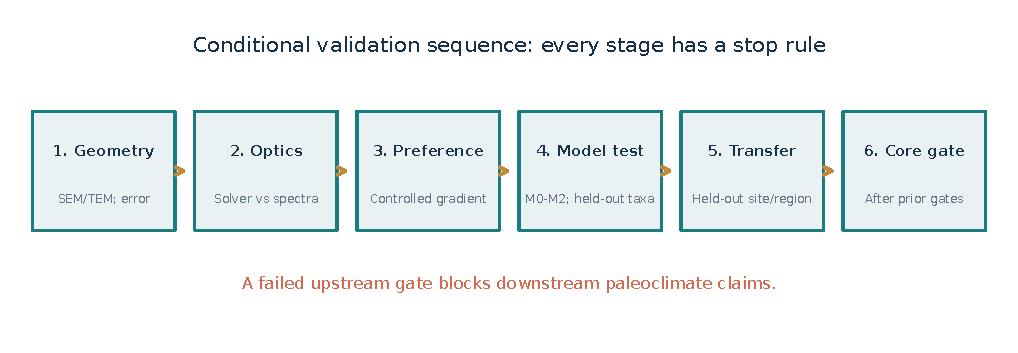
\includegraphics[width=0.96\linewidth]{figures/fig07_validation_flow.pdf}
\caption{Validation pipeline from geometry measurements to the pale-core gate. Later stages are conditional on earlier gates; a failure should stop downstream interpretation.}
\label{fig:flow1}
\end{figure}

\begin{figure}[H]
\centering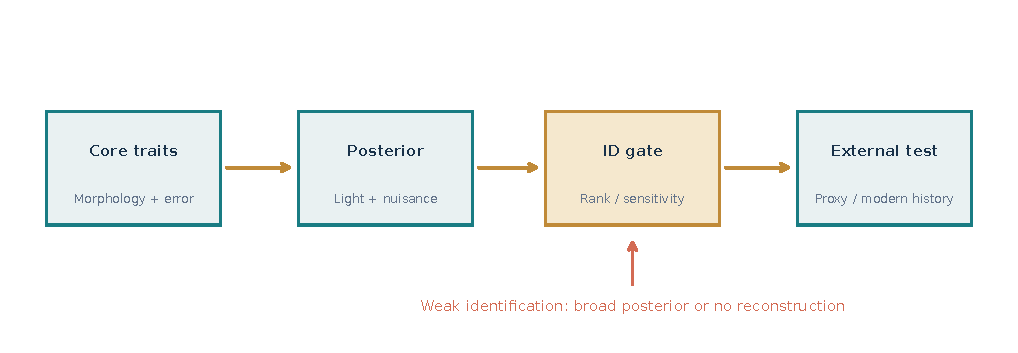
\includegraphics[width=0.96\linewidth]{figures/fig08_fail_closed_flow.pdf}
\caption{Fail-closed release and inference logic. Weak identification or failed calibration leads to a broad posterior, restricted claim or no reconstruction rather than a forced point estimate.}
\label{fig:flow2}
\end{figure}

\section{Proposed empirical programme}
\subsection{Stage A: calibration with extant species}
Select a phylogenetically stratified set of cultured taxa spanning centric/pennate lineages and a range of pore lattices, habitats and available light conditions. Sample multiple strains/populations where possible. Record taxonomy, sequence markers and provenance; calibrate microscopy and segmentation; measure frustule transmission/reflectance spectra under defined wavelengths, orientations, polarization and hydration/cleaning conditions. Compare the physical forward solver with measured spectra before extracting any ecological feature.

For each species, measure a pre-registered light-preference or performance endpoint in controlled light gradients, with randomized chamber positions, replicate cultures, standardized acclimation, temperature/nutrient controls, and independent sensor calibration. A growth-rate optimum, photosynthetic yield curve and survival threshold are distinct response variables; choose one primary endpoint before analysis and label others secondary. Avoid defining ``preference'' from the same optical formula that is subsequently used to predict it.

\subsection{Stage B: phylogenetic out-of-sample test}
Freeze the phylogeny or distribution over plausible trees; fit M0--M3 with outer folds split by taxon and an additional external validation split by site/region. Feature engineering, hyperparameter selection, thresholding and optical-feature compression must occur within training folds. Report held-out log predictive density, RMSE or a likelihood-appropriate score, calibration/coverage, uncertainty intervals and the incremental difference M2--M1. Use clade-preserving response permutations and simulated nulls to establish false-positive behaviour. A gain in random-fold validation but not held-out taxa or sites is not sufficient.

\subsection{Stage C: controlled light, UV and morphology perturbation}
Expose selected non-hazardous cultured diatoms to a factorial light-intensity/spectral-quality design, with UV treatment only where biologically and instrumentally justified. Test whether frustule geometry changes with the environment during growth, rather than assuming every interspecific difference is adaptive. Measure growth, viability, photosynthetic response, ultrastructure and the same optical features at baseline and after treatment. Distinguish plasticity within a lineage from multigenerational selection; the former does not alone demonstrate an evolutionary paleo-signal.

\subsection{Stage D: cores with independent constraints}
Only after stages A--C pass should a core reconstruction be attempted. Prioritize varved or annually resolved lakes with independent records of turbidity/water transparency, ice-cover duration, water level or catchment disturbance; modern instrumented lakes offer a calibration bridge. Pair sediment intervals with diatom assemblage composition, geometric measurements, chronology ensembles and independent environmental data. A core-only correlation between inferred light and another proxy from the same assemblage is not independent validation. For marine cores, address lateral transport, sediment focusing, reworking and the possibility that preservation selects particular morphotypes.

\begin{table}[H]
\caption{Falsification and stop criteria. The programme is designed so that failure remains interpretable.}
\label{tab:falsify}
\small\begin{tabularx}{\linewidth}{@{}p{0.31\linewidth}p{0.35\linewidth}X@{}}
\toprule
Observed outcome & Interpretation & Required response \\
\midrule
Optical solver fails measured-spectrum calibration & Geometry or optical constants are inadequate & Repair the forward model; do not run inverse learning \\
M2 does not outperform M1 after phylogeny/habitat controls & Spectral descriptors add no demonstrated incremental value & Report the null; retain simpler morphology baseline \\
Gain disappears for held-out taxa or region & Apparent association is local or ancestry-dependent & Restrict scope; seek more calibration coverage \\
Posterior changes sharply across reasonable attenuation priors & Target and nuisance are weakly identified & Report non-identifiability; withhold point reconstruction \\
Independent light proxy contradicts posterior at a rate beyond calibrated uncertainty & Inverse model is misspecified or uncalibrated & Stop the paleo claim; revise or reject the model \\
Morphology changes little under controlled light, or changes track nutrients/temperature instead & Proposed selection path is weak or confounded & Revise mechanism; do not assume light adaptation \\
\bottomrule\end{tabularx}
\end{table}

\section{Limitations, risks and interpretation}
The principal risk is equifinality: distinct histories can produce similar modern or fossil valve metrics. Spectral calculations do not solve this because different structures can have similar spectra, while identical structures under different water-column histories receive different illumination. Traits may also correlate with temperature, nutrients, iron, salinity, mechanical stress or species turnover. Tree uncertainty, misidentification, size diminution during the diatom life cycle, valve fragmentation, silica dissolution, sediment mixing and differential preservation can further perturb the proxy.

A second risk is confusing optical functionality with historical adaptation. A photonic effect measured in a present-day valve could be a consequence of geometry rather than an evolved response to a specific irradiance regime. Evidence of light focusing alone does not show that morphology evolved because of the light climate, and evidence of modern plasticity does not establish a million-year proxy transfer function. Each causal step requires a distinct test.

A third risk is inverse-model confidence. If the measured trait vector does not distinguish light from nuisance variables, a high-capacity generative model may still return a narrow posterior due to learned priors. Calibration must be assessed under synthetic prior-predictive checks, simulated misspecification, held-out modern sites, and sensitivity to prior and phylogeny. Uncertainty intervals cannot compensate for the absence of an independent target.

The project may still be useful if the central pale-light inversion fails. It could yield a calibrated database of species-specific photonic structures, identify optical traits that predict growth under contemporary controlled lighting, or demonstrate that pore-size associations are explained by phylogeny and habitat rather than light. These are narrower outcomes than a general deep-time light meter.

\section{Conclusion}
Silica Light Meters is a testable proposal, not a demonstrated proxy. Existing work establishes that diatom frustules can have wavelength-dependent optical effects and that morphology can covary with environmental conditions. The open test is whether a calibrated physics-derived descriptor adds out-of-sample information after phylogenetic and habitat controls, and whether that association remains measurable and identifiable in sediment cores. The workflow therefore begins with solver calibration and a nested species-level comparison, requires independent validation, and stops when the posterior is not identified. A negative result would be scientifically useful: it would set a boundary on what frustule geometry can be asked to reconstruct.

\section*{Research-process credit and AI disclosure}
Co-equal research-process credit is given to Devanik Debnath and Xylia, the autonomous multi-model research engine coordinating AI-assisted discovery, synthesis, and verification. Devanik Debnath retains responsibility for the final manuscript, scientific claims, citations, and released artifacts. Xylia is an AI research-orchestration system, not a human author.

\section*{Reproducibility and data availability}
All new numerical data in this release are synthetic outputs generated by \texttt{verify\_model.py}; generation assumptions and current-run outputs are archived in \texttt{results/}. No real species dataset, measured spectrum, phylogenetic tree or sediment core was analyzed. Reproduction commands and dependency information are in the repository README. The synthetic code tests pipeline logic, not biological claims.

\printbibliography[title={References}]
\end{document}
